\documentclass{article}

\usepackage{graphicx}
\usepackage{rotating}
\usepackage{amsmath}
\usepackage{amssymb}
\usepackage{mathrsfs}
\usepackage{fancyhdr}
\usepackage{listings}
\usepackage{xcolor}
\usepackage{color}
\usepackage{amsfonts}
\usepackage{textcomp}
\usepackage{float}
\usepackage{neuralnetwork}
\usepackage[sorting=none]{biblatex}
\usepackage[margin=1in]{geometry}
\usepackage[font={small,it}]{caption}
\usepackage{placeins}
\usepackage{xepersian}

%\DeclareMathOperator*{\btie}{\bowtie}
\addbibresource{bibliography.bib}
\settextfont[Scale=1.2]{B-NAZANIN.TTF}
\setlatintextfont[Scale=1]{Times New Roman}
\renewcommand{\baselinestretch}{1.5}
\pagestyle{fancy}
\fancyhf{}
\rhead{تکلیف اول درس یادگیری عمیق}
\lhead{\thepage}
\rfoot{علیرضا ابره فروش}
\lfoot{9816603}
\renewcommand{\headrulewidth}{1pt}
\renewcommand{\footrulewidth}{1pt}
\newcommand{\Lagr}{\mathcal{L}}
\newcommand{\Mod}[1]{\ (\mathrm{mod}\ #1)}
%%%%%%%%%%
\lstset
{
    language=[latex]tex,
    basicstyle=\ttfamily,
    commentstyle=\color{black},
    columns=fullflexible,
    keepspaces=true,
    upquote=true,
    showstringspaces=false,
    morestring=[s]\\\%,
    stringstyle=\color{black},
}
%%%%%%%%%%
%beginMatlab
\definecolor{mygreen}{RGB}{28,172,0} % color values Red, Green, Blue
\definecolor{mylilas}{RGB}{170,55,241}
%endMatlab
\begin{document}
%beginMatlab
\lstset{language=Matlab,%
    %basicstyle=\color{red},
    breaklines=true,%
    morekeywords={matlab2tikz},
    keywordstyle=\color{blue},%
    morekeywords=[2]{1}, keywordstyle=[2]{\color{black}},
    identifierstyle=\color{black},%
    stringstyle=\color{mylilas},
    commentstyle=\color{mygreen},%
    showstringspaces=false,%without this there will be a symbol in the places where there is a space
    numbers=left,%
    numberstyle={\tiny \color{black}},% size of the numbers
    numbersep=9pt, % this defines how far the numbers are from the text
    emph=[1]{for,end,break},emphstyle=[1]\color{red}, %some words to emphasise
    %emph=[2]{word1,word2}, emphstyle=[2]{style},    
}
%endMatlab
\begin{titlepage}
\begin{center}
\includegraphics[width=0.4\textwidth]{IUT Logo.png}\\
        
\LARGE
\textbf{دانشگاه صنعتی اصفهان}\\
\textbf{دانشکده مهندسی برق و کامپیوتر}\\
        
\vfill
        
\huge
\textbf{عنوان: تکلیف اول درس سیستم‌های عامل 1}\\
        
\vfill
        
\LARGE
\textbf{نام و نام خانوادگی: علیرضا ابره فروش}\\
\textbf{شماره دانشجویی: 9816603}\\
\textbf{نیم\,سال تحصیلی: پاییز 1400}\\
\textbf{مدرّس: دکتر محمّدرضا حیدرپور}\\
\textbf{دستیاران آموزشی: مجید فرهادی - دانیال مهرآیین - محمّد نعیمی}\\
\end{center}
\end{titlepage}


%\tableofcontents
\newpage


%1
\section{}
%$
%m = (00110010)_2 = (50)_{10} \\
%p = 23, q = 19 \\
%n = pq = 23 \times 19 = 437 \\
%z = (p-1)(q-1) = 22 \times 18 = 396 \\
%e = 97 \Rightarrow  e < n,\: (e, z) = 1 \\
%d = 49 \Rightarrow ed \equiv 1 (mod\:z) \\ \\
%c = (m ^ e \equiv 1 (mod \: n)) \Rightarrow c = 335 \\
%m = (c ^ d \equiv 1 (mod \: n)) \Rightarrow m = 50 \\ \\
%K^+ = e = 97 \\
%K^- = d = 49 \\
%$


%2
\section{}
%\lr{Trudy} می‌تواند به سیستم نفوذ کند و محتوای ارسال شده را تغییر دهد. به این صورت که $M$ و $H(M) + S$ را از هم جدا می‌کند. سپس با محاسبه‌ی \lr{hash}ِ پیامِ $M$ و حذف آن از $H(M)+S$ (به شکل $H(M) + S - H(M)$) به \lr{shared secret} دست پیدا می‌کند. سپس پیام مورد نظر خود ($M^{\prime}$) را به همراه $H(M^{\prime})$ و $S$ برای فرد به شکل
%$\left( M^{\prime}, H(M^{\prime}) + S \right)$
%ارسال می‌کند. با اینکه این پروتکل قابلیت نفوذ دارد اما به هر حال نمودار استخراج و \lr{Authentication}ِ پیام به صورت زیر است.
%\begin{figure}[H]
%    \centering
%    \includegraphics[width=0.50\textwidth]{figures/1.png}
%    \caption
%	{
%نمودار رمزگشایی پیام
%	}
%    \label{fig:fig1}
%\end{figure}


%3
\section{}
\subsection{الف}
تابع تانژانت هایپربولیک ($tanh$) اغلب به عنوان نسخه مقیاس‌شده‌ای از تابع سیگموید توصیف می‌شود، به خصوص تابع سیگموید لجستیک. این رابطه به دلیل شباهت‌های تابع تانژانت و تابع سیگموید وجود دارد، اما در بازه و مقیاس‌شان تفاوت دارند.\\
تابع سیگموید که اغلب با نماد $\sigma\left( x \right)$ نشان داده می‌شود، به شرح زیر تعریف می‌شود:
\begin{latin}
$
\sigma\left( x \right) = \frac{1}{1 + e ^ {-x}}
$
\end{latin}
این تابع هر عدد حقیقی را به یک مقدار بین 0 و 1 نگاشت می‌کند. وقتی $x$ یک عدد مثبت بزرگ است، $\sigma\left( x \right)$ به 1 نزدیک می‌شود و وقتی $x$ یک عدد منفی بزرگ است، $\sigma\left( x \right)$ به 0 نزدیک می‌شود. این به این معناست که تابع سیگموید ورودی خود را در بازه (0، 1) فشرده می‌کند که برای مسائل دسته‌بندی دودویی مفید است، چون می‌توان از آن تعبیر احتمالاتی کرد.\\
تابع تانژانت هایپربولیک، به شکل زیر تعریف می‌شود:
\begin{latin}
$
tanh(x) = \frac{e^x - e^{-x}}{e^x + e^{-x}} = \frac{e ^ {2x} - 1}{e ^ {2x} + 1}
$
\end{latin}
تابع تانژانت هایپربولیک هر عدد حقیقی را به یک مقدار بین 1- و 1 نگاشت می‌دهد. وقتی $x$ یک عدد مثبت بزرگ است، $tanh(x)$ به 1 نزدیک می‌شود و وقتی $x$ یک عدد منفی بزرگ است، $tanh(x)$ به 1- نزدیک می‌شود.\\

رابطه بین توابع تانژانت هایپربولیک و سیگموید به شرح زیر است:
\begin{enumerate}
\item مقیاس‌دهی: تابع تانژانت هایپربولیک، انتقال داده شده و مقیاس شده‌ی تابع سیگموید به منظور داشتن رنج $(-1, 1)$ به جای $(0, 1)$ است. این مقیاس‌دهی با کم کردن $0.5$ از تابع سیگموید و سپس ضرب آن در 2 انجام می‌شود:
\begin{latin}
$
2\sigma\left( 2x \right)-1 = 
2 \times \frac{1}{1 + e ^ {-2x}} - 1 =
\frac{1 - e ^ {-2x}}{1 + e ^ {-2x}} = 
\frac{1 - e ^ {-2x}}{1 + e ^ {-2x}} \times \frac{e ^ {2x}}{e ^ {2x}} =
\frac{e ^ {2x} - 1}{e ^ {2x} + 1} = tanh\left( x \right)\\ \Rightarrow 
tanh(x) = 2\sigma\left( 2x \right) - 1
$
\end{latin}

\item تقارن: یکی از تفاوت‌های کلیدی این است که تابع تانژانت هایپربولیک در اطراف مبدأ متقارن است (در واقع $tanh(-x) = -tanh(x)$)، درحالی که تابع سیگموید این تقارن را ندارد.

\end{enumerate}
تابع تانژانت هایپربولیک اغلب به عنوان یک جایگزین برای تابع سیگموید در شبکه‌های عصبی استفاده می‌شود. زیرا به دلیل ماهیت مرکز شده حول صفری که دارد، یادگیری در شبکه‌های عمیق را سریع‌تر می‌کند. اینکه تابع تانژانت هایپربولیک مقادیر منفی را نیز خروجی دهد به معنای این است که می‌تواند تغییرات مثبت و منفی را در واحدهای مخفی شبکه در طول آموزش ایجاد کند که می‌تواند به همگرایی کمک کند. با این حال، هر دو تابع هنوز در متنوعی از زمینه‌ها استفاده می‌شوند و انتخاب بین آن‌ها بستگی به مسئله خاص و معماری شبکه دارد.



\subsection{ب}
\begin{latin}
$
p\left( x \right) = x \log\left( 1 + tanh\left( e ^ {x} \right) \right)\\ \\
\frac{d}{dx} p\left( x \right) = \left( \frac{d}{dx}x \right) \times \log\left( 1 + tanh\left( e ^ {x} \right) \right) +
\left( \frac{d}{dx}\left( \log\left( 1 + tanh\left( e ^ {x} \right) \right) \right) \right) \times x \\=
\log\left( 1 + tanh\left( e ^ {x} \right) \right) + 
x\left( \frac{d }{dx}\left( 1 + tanh\left( e ^ {x} \right) \right) \right) \times \frac{1}{1 + tanh\left( e ^ {x} \right)}
\\= \log\left( 1 + tanh\left( e ^ {x} \right) \right) +
\frac{x}{1 + tanh\left( e ^ {x} \right)} \times \left( \frac{d }{dx}\left( tanh\left( e ^ {x} \right) \right) \right)
\\= \log\left( 1 + tanh\left( e ^ {x} \right) \right) + \frac{x}{1 + tanh\left( e ^ {x} \right)} \times 
\left( \frac{d }{dx}\left( e ^ {x} \right) \right) \times \left( 1 - tanh^2\left( e ^ x \right) \right)
\\=
\log\left( 1 + tanh\left( e ^ {x} \right) \right) + 
xe^x\left( 1 - tanh\left( e ^ x \right) \right)
$
\end{latin}

%4
\section{}
\begin{latin}
\begin{neuralnetwork}[height=9]
    \newcommand{\x}[2]{$x_#2$}
    \newcommand{\y}[2]{$\hat{y}_#2$}
    \newcommand{\hfirst}[2]{\small $h^{(1)}_#2$}
    \newcommand{\hsecond}[2]{\small $h^{(2)}_#2$}
    \inputlayer[count=4, bias=true, title=Input\\layer, text=\x]
    \hiddenlayer[count=7, bias=true, title=Hidden\\layer, text=\hfirst] \linklayers
    \outputlayer[count=3, title=Output\\layer, text=\y] \linklayers
\end{neuralnetwork}
\end{latin}
با توجه به شبکه‌ی بالا، نورون‌های سبز، بنفش، و قرمز به ترتیب لایه‌ی ورودی، لایه‌ی مخفی، و لایه‌ی خروجی را تشکیل می‌دهند و همچنین نورون‌های زرد \lr{bias}ها هستند که همگی مقدار 1 دارند. پارامترهای قابل یادگیری شبکه وزن‌های موجود بین نورون‌هاست که تعدادشان برابر است با:
$
4 \times 7 + 7 + 7 \times 3 + 3 = 59
$


%5
\section{}

\begin{latin}
\begin{neuralnetwork}[height=4, layerspacing=20mm, nodespacing=15mm, maintitleheight=2.5em, layertitleheight=2.5em]
    \newcommand{\x}[2]{$x_#2$}
    \newcommand{\relu}[2]{\small $a_#2$}
    \newcommand{\y}[2]{$\hat{y}$}
    \inputlayer[count=2, bias=false, title=Input Layer, text=\x]
    \hiddenlayer[count=3, bias=false, title=ReLU Layer, text=\relu] \linklayers
    \outputlayer[count=1, title=Output Layer, text=\y] \linklayers
\end{neuralnetwork}
\end{latin}

\begin{latin}
$
J\left( W \right) = \frac{1}{n} \sum_{i = 1}^{n} L\left( \hat{y} ^ {( i )}, y ^ { ( i ) } \right) = \left( \hat{y} ^ {( 1 )} - y ^ {( 1 )} \right) ^ {2} = \left( \hat{y} - 3 \right) ^ {2}
\\
x = \begin{bmatrix}
x_1 \\
x_2
\end{bmatrix}
\\
z = \begin{bmatrix}
z_1 \\
z_2 \\
z_3
\end{bmatrix} =
\begin{bmatrix}
w_1 & w_2 \\
w_3 & w_4 \\
w_5 & w_6
\end{bmatrix}
x
\\
a = \begin{bmatrix}
a_1 \\
a_2 \\
a_3
\end{bmatrix} =
ReLU\left( z \right)
\\
z_4 =
\begin{bmatrix}
w_7 &
w_8 &
w_9
\end{bmatrix}a
\\
\hat{y} = ReLU\left( z_4 \right)
\\
\\
\\
\begin{bmatrix}
x_1 \\
x_2
\end{bmatrix}=
\begin{bmatrix}
1 \\
2
\end{bmatrix}
\\ y = 3
\\
\begin{bmatrix}
z_1 \\
z_2 \\
z_3
\end{bmatrix} =
\begin{bmatrix}
2 & 1 \\
1 & -2 \\
1 & 2
\end{bmatrix}
\begin{bmatrix}
1 \\
2
\end{bmatrix} =
\begin{bmatrix}
4 \\
-3 \\
5
\end{bmatrix}
\\ a = 
ReLU\left(
\begin{bmatrix}
4 \\
-3 \\
5
\end{bmatrix}
\right) =
\begin{bmatrix}
4 \\
0 \\
5
\end{bmatrix}
\\
z_4 = 
\begin{bmatrix}
-1 &
3 &
2
\end{bmatrix}
\begin{bmatrix}
4 \\
0 \\
5
\end{bmatrix} = 6
\\
\hat{y} = ReLU\left( 6 \right) = 6
\\
\\
\\
\begin{bmatrix}
w_7 &
w_8 &
w_9
\end{bmatrix}
\gets 
\begin{bmatrix}
w_7 &
w_8 &
w_9
\end{bmatrix}
-\alpha
\begin{bmatrix}
\frac{\partial J\left( W \right)}{\partial w_7} &
\frac{\partial J\left( W \right)}{\partial w_8} &
\frac{\partial J\left( W \right)}{\partial w_9}
\end{bmatrix} 
\\ =
\begin{bmatrix}
-1 &
3 &
2
\end{bmatrix}
-0.1
\begin{bmatrix}
\frac{\partial J\left( W \right)}{\partial \hat{y}} \times \frac{\partial \hat{y}}{\partial w_7} &
\frac{\partial J\left( W \right)}{\partial \hat{y}} \times \frac{\partial \hat{y}}{\partial w_8} &
\frac{\partial J\left( W \right)}{\partial \hat{y}} \times \frac{\partial \hat{y}}{\partial w_9}
\end{bmatrix}
\\=
\begin{bmatrix}
-1 &
3 &
2
\end{bmatrix}
-0.1
\begin{bmatrix}
2\left( \hat{y} - y \right)a_1 &
2\left( \hat{y} - y \right)a_2 &
2\left( \hat{y} - y \right)a_3
\end{bmatrix}
\\=
\begin{bmatrix}
-1 &
3 &
2
\end{bmatrix}
-0.1
\begin{bmatrix}
24 &
0 &
30
\end{bmatrix} = \begin{bmatrix}
-3.4 &
3 &
-1
\end{bmatrix}
\\ \\ 
\begin{bmatrix}
w_1 & w_2 \\
w_3 & w_4 \\
w_5 & w_6
\end{bmatrix}
\gets 
\begin{bmatrix}
w_1 & w_2 \\
w_3 & w_4 \\
w_5 & w_6
\end{bmatrix}
-\alpha
\begin{bmatrix}
\frac{\partial J\left( W \right)}{\partial w_1} & \frac{\partial J\left( W \right)}{\partial w_2} \\
\frac{\partial J\left( W \right)}{\partial w_3} & \frac{\partial J\left( W \right)}{\partial w_4} \\
\frac{\partial J\left( W \right)}{\partial w_5} & \frac{\partial J\left( W \right)}{\partial w_6}
\end{bmatrix}
\\=
\begin{bmatrix}
2 & 1 \\
1 & -2 \\
1 & 2
\end{bmatrix}
-0.1
\begin{bmatrix}
\frac{\partial J\left( W \right)}{\partial \hat{y}} \times \frac{\partial \hat{y}}{\partial a_1} \times \frac{\partial a_1}{\partial z_1} \times \frac{\partial z_1}{\partial w_1}
&
\frac{\partial J\left( W \right)}{\partial \hat{y}} \times \frac{\partial \hat{y}}{\partial a_1} \times \frac{\partial a_1}{\partial z_1} \times \frac{\partial z_1}{\partial w_2}
\\
\frac{\partial J\left( W \right)}{\partial \hat{y}} \times \frac{\partial \hat{y}}{\partial a_2} \times \frac{\partial a_2}{\partial z_2} \times \frac{\partial z_2}{\partial w_3}
&
\frac{\partial J\left( W \right)}{\partial \hat{y}} \times \frac{\partial \hat{y}}{\partial a_2} \times \frac{\partial a_2}{\partial z_2} \times \frac{\partial z_2}{\partial w_4}
\\
\frac{\partial J\left( W \right)}{\partial \hat{y}} \times \frac{\partial \hat{y}}{\partial a_3} \times \frac{\partial a_3}{\partial z_3} \times \frac{\partial z_3}{\partial w_5}
&
\frac{\partial J\left( W \right)}{\partial \hat{y}} \times \frac{\partial \hat{y}}{\partial a_3} \times \frac{\partial a_3}{\partial z_3} \times \frac{\partial z_3}{\partial w_6}
\end{bmatrix}
\\=
\begin{bmatrix}
2 & 1 \\
1 & -2 \\
1 & 2
\end{bmatrix}
-0.1
\begin{bmatrix}
2\left( \hat{y} - y \right) \times w_7 \times 1 \times x_1
&
2\left( \hat{y} - y \right) \times w_7 \times 1 \times x_2
\\
2\left( \hat{y} - y \right) \times w_8 \times 0 \times x_1
&
2\left( \hat{y} - y \right) \times w_8 \times 0 \times x_2
\\
2\left( \hat{y} - y \right) \times w_9 \times 1 \times x_1
&
2\left( \hat{y} - y \right) \times w_9 \times 1 \times x_2
\end{bmatrix}
\\=
\begin{bmatrix}
2 & 1 \\
1 & -2 \\
1 & 2
\end{bmatrix}
-0.1
\begin{bmatrix}
-6
&
-12
\\
0
&
0
\\
12
&
36
\end{bmatrix} =
\begin{bmatrix}
2.6 & 2.2 \\
1 & -2 \\
-0.2 & -1.6
\end{bmatrix}
$
\end{latin}


%6
\section{}
\subsection{الف}
\begin{latin}


\tikzset{every picture/.style={line width=0.75pt}} %set default line width to 0.75pt        

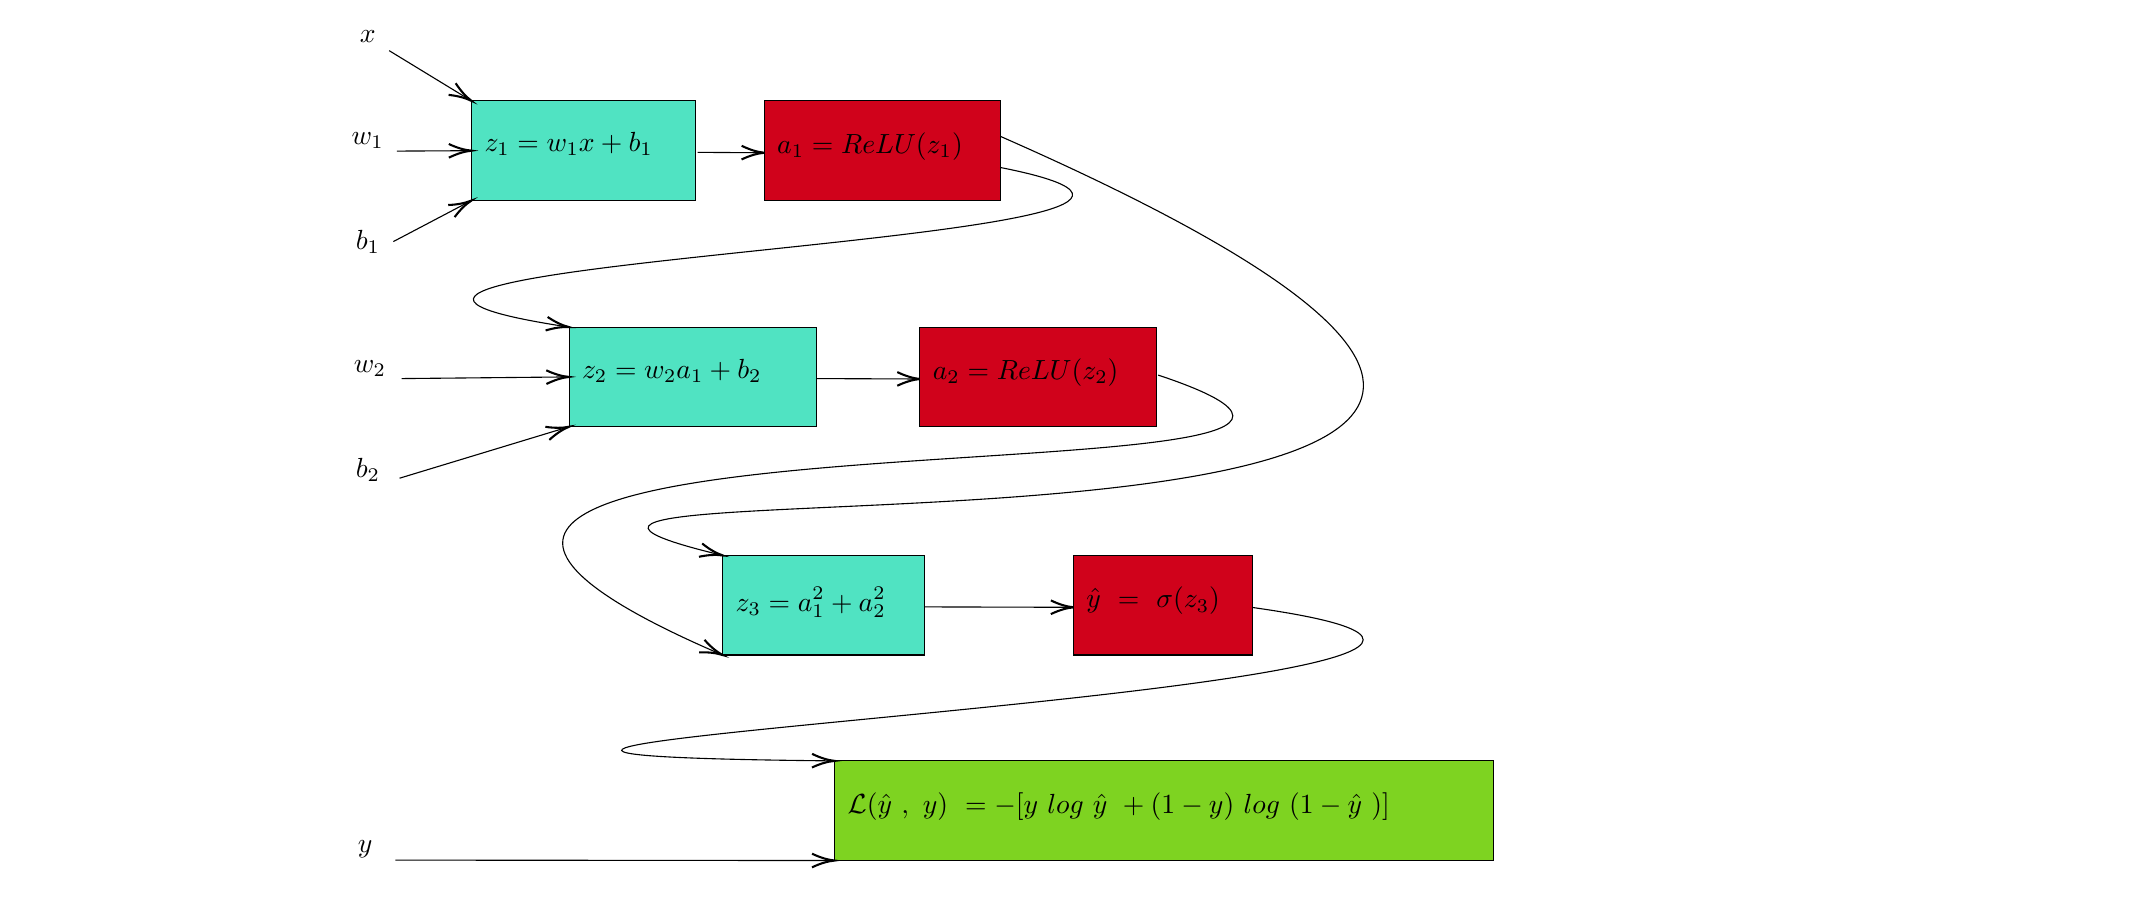
\begin{tikzpicture}[x=0.75pt,y=0.75pt,yscale=-1,xscale=1]
%uncomment if require: \path (0,433); %set diagram left start at 0, and has height of 433

%Shape: Rectangle [id:dp26082320028943795] 
\draw  [fill={rgb, 255:red, 80; green, 227; blue, 194 }  ,fill opacity=1 ] (62,46) -- (170.07,46) -- (170.07,94) -- (62,94) -- cycle ;
%Straight Lines [id:da5321728940522126] 
\draw    (22.33,21.8) -- (60.29,44.96) ;
\draw [shift={(62,46)}, rotate = 211.39] [color={rgb, 255:red, 0; green, 0; blue, 0 }  ][line width=0.75]    (10.93,-3.29) .. controls (6.95,-1.4) and (3.31,-0.3) .. (0,0) .. controls (3.31,0.3) and (6.95,1.4) .. (10.93,3.29)   ;
%Straight Lines [id:da8722522064456113] 
\draw    (26.07,70.2) -- (60,70.01) ;
\draw [shift={(62,70)}, rotate = 179.68] [color={rgb, 255:red, 0; green, 0; blue, 0 }  ][line width=0.75]    (10.93,-3.29) .. controls (6.95,-1.4) and (3.31,-0.3) .. (0,0) .. controls (3.31,0.3) and (6.95,1.4) .. (10.93,3.29)   ;
%Straight Lines [id:da4977170317452869] 
\draw    (24.33,113.8) -- (60.23,94.93) ;
\draw [shift={(62,94)}, rotate = 152.27] [color={rgb, 255:red, 0; green, 0; blue, 0 }  ][line width=0.75]    (10.93,-3.29) .. controls (6.95,-1.4) and (3.31,-0.3) .. (0,0) .. controls (3.31,0.3) and (6.95,1.4) .. (10.93,3.29)   ;
%Straight Lines [id:da9786960106080183] 
\draw    (171,70.8) -- (201.07,70.99) ;
\draw [shift={(203.07,71)}, rotate = 180.36] [color={rgb, 255:red, 0; green, 0; blue, 0 }  ][line width=0.75]    (10.93,-3.29) .. controls (6.95,-1.4) and (3.31,-0.3) .. (0,0) .. controls (3.31,0.3) and (6.95,1.4) .. (10.93,3.29)   ;
%Shape: Rectangle [id:dp4699732294865028] 
\draw  [fill={rgb, 255:red, 208; green, 2; blue, 27 }  ,fill opacity=1 ] (203,46) -- (317.07,46) -- (317.07,94) -- (203,94) -- cycle ;
%Shape: Rectangle [id:dp7233773663060797] 
\draw  [fill={rgb, 255:red, 80; green, 227; blue, 194 }  ,fill opacity=1 ] (109,155) -- (228.33,155) -- (228.33,203) -- (109,203) -- cycle ;
%Straight Lines [id:da5907930980218636] 
\draw    (28.33,179.8) -- (107,179.02) ;
\draw [shift={(109,179)}, rotate = 179.43] [color={rgb, 255:red, 0; green, 0; blue, 0 }  ][line width=0.75]    (10.93,-3.29) .. controls (6.95,-1.4) and (3.31,-0.3) .. (0,0) .. controls (3.31,0.3) and (6.95,1.4) .. (10.93,3.29)   ;
%Straight Lines [id:da5935250653594418] 
\draw    (27.33,227.8) -- (107.09,203.58) ;
\draw [shift={(109,203)}, rotate = 163.11] [color={rgb, 255:red, 0; green, 0; blue, 0 }  ][line width=0.75]    (10.93,-3.29) .. controls (6.95,-1.4) and (3.31,-0.3) .. (0,0) .. controls (3.31,0.3) and (6.95,1.4) .. (10.93,3.29)   ;
%Straight Lines [id:da4807719277385877] 
\draw    (228.33,179.8) -- (276.07,179.99) ;
\draw [shift={(278.07,180)}, rotate = 180.23] [color={rgb, 255:red, 0; green, 0; blue, 0 }  ][line width=0.75]    (10.93,-3.29) .. controls (6.95,-1.4) and (3.31,-0.3) .. (0,0) .. controls (3.31,0.3) and (6.95,1.4) .. (10.93,3.29)   ;
%Shape: Rectangle [id:dp004733566676465184] 
\draw  [fill={rgb, 255:red, 208; green, 2; blue, 27 }  ,fill opacity=1 ] (278,155) -- (392.07,155) -- (392.07,203) -- (278,203) -- cycle ;
%Curve Lines [id:da43051210766963555] 
\draw    (316.83,78.1) .. controls (498.83,114.1) and (-103.67,122.8) .. (109,155) ;
\draw [shift={(109,155)}, rotate = 188.61] [color={rgb, 255:red, 0; green, 0; blue, 0 }  ][line width=0.75]    (10.93,-3.29) .. controls (6.95,-1.4) and (3.31,-0.3) .. (0,0) .. controls (3.31,0.3) and (6.95,1.4) .. (10.93,3.29)   ;
%Shape: Rectangle [id:dp7844392260191501] 
\draw  [fill={rgb, 255:red, 80; green, 227; blue, 194 }  ,fill opacity=1 ] (183,265) -- (280.33,265) -- (280.33,313) -- (183,313) -- cycle ;
%Straight Lines [id:da7438844634576284] 
\draw    (280.33,289.8) -- (350.07,289.99) ;
\draw [shift={(352.07,290)}, rotate = 180.16] [color={rgb, 255:red, 0; green, 0; blue, 0 }  ][line width=0.75]    (10.93,-3.29) .. controls (6.95,-1.4) and (3.31,-0.3) .. (0,0) .. controls (3.31,0.3) and (6.95,1.4) .. (10.93,3.29)   ;
%Shape: Rectangle [id:dp06514973867064988] 
\draw  [fill={rgb, 255:red, 208; green, 2; blue, 27 }  ,fill opacity=1 ] (352,265) -- (438.33,265) -- (438.33,313) -- (352,313) -- cycle ;
%Curve Lines [id:da5234327252277915] 
\draw    (316.83,63.1) .. controls (853.83,299.1) and (-37.87,212.1) .. (183,265) ;
\draw [shift={(183,265)}, rotate = 193.47] [color={rgb, 255:red, 0; green, 0; blue, 0 }  ][line width=0.75]    (10.93,-3.29) .. controls (6.95,-1.4) and (3.31,-0.3) .. (0,0) .. controls (3.31,0.3) and (6.95,1.4) .. (10.93,3.29)   ;
%Curve Lines [id:da12663621077553533] 
\draw    (392.83,178.1) .. controls (593.17,244.9) and (-122.67,181.8) .. (183,313) ;
\draw [shift={(183,313)}, rotate = 203.23] [color={rgb, 255:red, 0; green, 0; blue, 0 }  ][line width=0.75]    (10.93,-3.29) .. controls (6.95,-1.4) and (3.31,-0.3) .. (0,0) .. controls (3.31,0.3) and (6.95,1.4) .. (10.93,3.29)   ;
%Shape: Rectangle [id:dp1997427400696722] 
\draw  [fill={rgb, 255:red, 126; green, 211; blue, 33 }  ,fill opacity=1 ] (237,364) -- (554.43,364) -- (554.43,412) -- (237,412) -- cycle ;
%Straight Lines [id:da05813852175573886] 
\draw    (25.33,411.8) -- (235,412) ;
\draw [shift={(237,412)}, rotate = 180.05] [color={rgb, 255:red, 0; green, 0; blue, 0 }  ][line width=0.75]    (10.93,-3.29) .. controls (6.95,-1.4) and (3.31,-0.3) .. (0,0) .. controls (3.31,0.3) and (6.95,1.4) .. (10.93,3.29)   ;
%Curve Lines [id:da6379195786923225] 
\draw    (438.43,290.1) .. controls (707.43,328.1) and (-151.57,360.1) .. (237,364) ;
\draw [shift={(237,364)}, rotate = 180.58] [color={rgb, 255:red, 0; green, 0; blue, 0 }  ][line width=0.75]    (10.93,-3.29) .. controls (6.95,-1.4) and (3.31,-0.3) .. (0,0) .. controls (3.31,0.3) and (6.95,1.4) .. (10.93,3.29)   ;

% Text Node
\draw (67,60) node [anchor=north west][inner sep=0.75pt]   [align=left] {$\displaystyle z_{1} =w_{1} x+b_{1}$};
% Text Node
\draw (7,11) node [anchor=north west][inner sep=0.75pt]   [align=left] {$\displaystyle x$};
% Text Node
\draw (3,60) node [anchor=north west][inner sep=0.75pt]   [align=left] {$\displaystyle w_{1}$};
% Text Node
\draw (5,107) node [anchor=north west][inner sep=0.75pt]   [align=left] {$\displaystyle b_{1}$};
% Text Node
\draw (208,60) node [anchor=north west][inner sep=0.75pt]   [align=left] {$\displaystyle a_{1} =ReLU( z_{1})$};
% Text Node
\draw (114,169) node [anchor=north west][inner sep=0.75pt]   [align=left] {$\displaystyle z_{2} =w_{2} a_{1} +b_{2}$};
% Text Node
\draw (4,170) node [anchor=north west][inner sep=0.75pt]   [align=left] {$\displaystyle w_{2}$};
% Text Node
\draw (5,217) node [anchor=north west][inner sep=0.75pt]   [align=left] {$\displaystyle b_{2}$};
% Text Node
\draw (283,169) node [anchor=north west][inner sep=0.75pt]   [align=left] {$\displaystyle a_{2} =ReLU( z_{2})$};
% Text Node
\draw (188,279) node [anchor=north west][inner sep=0.75pt]   [align=left] {$\displaystyle z_{3} =a_{1}^{2} +a_{2}^{2}$};
% Text Node
\draw (357,279) node [anchor=north west][inner sep=0.75pt]   [align=left] {$\displaystyle \hat{y} \ =\ \sigma ( z_{3})$};
% Text Node
\draw (242,378) node [anchor=north west][inner sep=0.75pt]   [align=left] {$\displaystyle \mathcal{L}(\hat{y} \ ,\ y) \ =-[ y\ log\ \hat{y} \ +( 1-y) \ log\ ( 1-\hat{y} \ )] \ $};
% Text Node
\draw (6,401) node [anchor=north west][inner sep=0.75pt]   [align=left] {$\displaystyle y$};


\end{tikzpicture}

\end{latin}


\subsection{ب}
\begin{latin}
$
\frac{\partial L}{\partial a_1} =
\frac{\partial L}{\partial \hat{y}} \times
\frac{\partial \hat{y}}{\partial z_3} \times
\frac{\partial z_3}{\partial a_1} =
\left(\frac{-y}{\hat{y}} + \frac{1-y}{1-\hat{y}}\right) \times
\hat{y}\left( 1-\hat{y} \right) \times
2a_1 =
\left( \hat{y} - y \right)2a_1
$
\\
\\
$
\frac{\partial L}{\partial a_2} =
\frac{\partial L}{\partial \hat{y}} \times
\frac{\partial \hat{y}}{\partial z_3} \times
\frac{\partial z_3}{\partial a_2} =
\left(\frac{-y}{\hat{y}} + \frac{1-y}{1-\hat{y}}\right) \times
\hat{y}\left( 1-\hat{y} \right) \times
2a_2 =
\left( \hat{y} - y \right)2a_2
$
\\
\\
$
\frac{\partial L}{\partial w_1} =
\frac{\partial L}{\partial \hat{y}} \times
\frac{\partial \hat{y}}{\partial z_3} \times
\left(
\frac{\partial z_3}{\partial a_1} \times \frac{\partial a_1}{\partial z_1} \times \frac{\partial z_1}{\partial w_1}            +
\frac{\partial z_3}{\partial a_2} \times \frac{\partial a_2}{\partial z_2} \times \frac{\partial z_2}{\partial a_1} \times \frac{\partial a_1}{\partial z_1} \times \frac{\partial z_1}{\partial w_1}
\right)
\\=
\frac{\partial L}{\partial a_1} \times \frac{\partial a_1}{\partial z_1} \times \frac{\partial z_1}{\partial w_1}
+
\frac{\partial L}{\partial a_2} \times \frac{\partial a_2}{\partial z_2} \times \frac{\partial z_2}{\partial a_1} \times \frac{\partial a_1}{\partial z_1} \times \frac{\partial z_1}{\partial w_1}
\\=
\left( \hat{y} - y \right)2a_1 \times a_1\left( 1 - a_1 \right) \times x
+
\left( \hat{y} - y \right)2a_2 \times a_2\left( 1 - a_2 \right) \times w_2 \times a_1\left( 1 - a_1 \right) \times x
\\=
2\left( \hat{y} - y \right)a_1\left( 1 - a_1 \right)x\left[ a_1 + a_2 ^ 2\left( 1 - a_2 \right) w_2 \right]
$
\end{latin}


%\begin{enumerate}
%	\item \lr{Bob} لیستی از الگوریتم‌هایی که از آن‌ها پشتیبانی می‌کند را به همراه \lr{nonce} به \lr{Alice} می‌فرستد.
%	\item \lr{Alice} بین لیست الگوریتم‌های پیشنهادی یکی را انتخاب می‌کند و آن را به همراه \lr{certificate} و \lr{nonce} می‌فرستد.
%	\item \lr{Bob} \lr{certificate} را اعتبارسنجی می‌کند، \lr{public key}ِ \lr{Alice} را استخراج می‌کند، \lr{pre\_master\_secret} را تولید می‌کند، با \lr{public key}ِ \lr{Alice} آن را رمز می‌کند و برای \lr{Alice} می‌فرستد.
%	\item \lr{Bob} و \lr{Alice} به طور مستقل رمز و کلیدهای \lr{MAC} را از \lr{pre\_master\_secret} و \lr{nonce}ها محاسبه می‌کنند.
%	\item \lr{Bob} یک \lr{MAC} از همه‌ی پیام‌های \lr{handshake} می‌فرستد.
%	\item \lr{Alice} یک \lr{MAC} از همه‌ی پیام‌های \lr{handshake} می‌فرستد.
%\end{enumerate}




%%%%%%%%%%%%%%%%%%%%%%%%%%%%%%%%%%%
%%%%%%%%%%%%%%%%%%%%%%%%%%%%%%%%%%%
%%%%%%%%%%%%%%%%%%%%%%%%%%%%%%%%%%%



\section*{منابع}
\renewcommand{\section}[2]{}%
\begin{thebibliography}{99} % assumes less than 100 references
%چنانچه مرجع فارسی نیز داشته باشید باید دستور فوق را فعال کنید و مراجع فارسی خود را بعد از این دستور وارد کنید


\begin{LTRitems}

\resetlatinfont

\bibitem{b1} Stošić, Lazar, and Milena Bogdanović. "RC4 stream cipher and possible attacks on WEP." Editorial Preface 3.3 (2012).
\end{LTRitems}

\end{thebibliography}


\end{document}
